\paragraph{QuizziPedia::Front-End::Services::UserDetailsService}

\label{QuizziPedia::Front-End::Services::UserDerailsService}
\begin{figure}[ht]
	\centering
	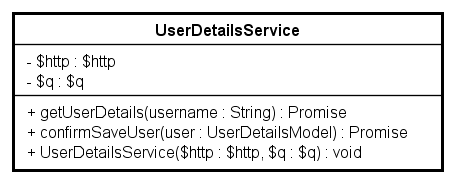
\includegraphics[scale=0.60]{UML/Classi/Front-End/QuizziPedia_Front-end_Services_UserDetailsService.png}
	\caption{QuizziPedia::Front-End::Services::UserDetailsService}
\end{figure}\FloatBarrier
\begin{itemize}
	\item \textbf{Descrizione}: questa classe permette di ottenere i dati personali degli utenti;
	\item \textbf{Utilizzo}: utilizzata per ottenere i dati personali di un utente. Permette inoltre di trovare i dati di utenti ricercati tramite l'apposita barra di ricerca;
	\item \textbf{Relazione con altre classi}:
	\begin{itemize}
		\item \textbf{IN \texttt{UserDetailsModel}}: rappresenta un utente. Contiene tutte le informazioni necessarie alla	presentazione del contenuto di un utente sia nella visualizzazione che nella gestione di un profilo; 
		\item \textbf{OUT \texttt{SearchController}}: questa classe permette di gestire la ricerca di questionari e utenti all'interno dell'applicazione;
		\item \textbf{OUT \texttt{UserDetailsController}}: questa classe permette di gestire i dati di un utente;
		\item \textbf{OUT \texttt{ProfileManagementController}}: questa classe permette di gestire il profilo personale di un utente. 
	\end{itemize}
	\item \textbf{Attributi}:
	\begin{itemize}
		\item \texttt{-} \texttt{\$http: \$http} \\ Campo dati che contiene un riferimento al servizio \$http che permette la comunicazione con il protocollo \textit{HTTP\ped{G}};
		\item \texttt{-} \texttt{\$q: \$q} \\ Campo dati che contiene un riferimento a \$q, un servizio offerto da \textit{Angular\ped{G}} per la gestione, tramite \textit{Promise\ped{G}}, di chiamate asincrone.
	\end{itemize}
	\item \textbf{Metodi}:
	\begin{itemize}
		\item \texttt{+} \texttt{UserDetailsService(\$http: \$http, \$q: \$q)} \\ Metodo costruttore della classe; \\
		\textbf{Parametri}:
		\begin{itemize}
			\item \texttt{\$http: \$http} \\ Campo dati che contiene un riferimento al servizio \$http che permette la comunicazione con il protocollo \textit{HTTP\ped{G}};
			\item \texttt{\$q: \$q} \\ Campo dati che contiene un riferimento a \$q, un servizio offerto da \textit{Angular\ped{G}} per la gestione, tramite \textit{Promise\ped{G}}, di chiamate asincrone.
		\end{itemize}
		\item \texttt{+} \texttt{getUserDetails(username: String): Promise} \\ Metodo che serve per ottenere i dettagli di un utente. Il metodo ritorna una \textit{Promise\ped{G}}. In caso la \textit{Promise\ped{G}} venga rifiutata, verrà restituito al \texttt{SearchController} un oggetto \texttt{ErrorModelInfo} contenente tutti i dettagli dell'errore. In caso la \textit{Promise\ped{G}} venga accettata, verrà restituito al chiamante del metodo il risultato della chiamata;\\
		\textbf{Parametri}:
		\begin{itemize}
			\item \texttt{username: String} \\ Parametro che indica l'utente del quale andranno caricati tutti i dati personali.
		\end{itemize}
		\item \texttt{+} \texttt{confirmSaveUser(user: Object, imageObject: Object): Promise} \\Metodo che serve per inviare al back-end una richiesta di salvataggio persistente dei dati. Viene invocato da \texttt{Confirm} in \texttt{ProfileManagementController}. Il metodo ritorna una \textit{Promise\ped{G}}. In caso la \textit{Promise\ped{G}} venga rifiutata, verrà restituito al \texttt{ProfileManagementController} un oggetto \texttt{ErrorModelInfo} contenente tutti i dettagli dell'errore. In caso la \textit{Promise\ped{G}} venga accettata, verrà restituito al chiamante del metodo il risultato della chiamata.\\
		\textbf{Parametri}:
		\begin{itemize}
			\item \texttt{user: Object} \\ Parametro che indica l'oggetto contenente tutti i dati dell'utente che dovranno essere salvati dal back-end;
			\item \texttt{imageObject: Object} \\ Oggetto contenente i seguenti attributi: \texttt{+ imageUrl: String}, \\ \texttt{+ image: Object}.
		\end{itemize}
	
	\end{itemize}
\end{itemize}
